\chapter{Study of Particle Multiplicity of Cosmic Ray Events using
  2\,m\,$\times$\,2\,m Resistive Plate Chamber Stack at IICHEP-Madurai}

One of the main goals of the INO Project is to collaborate with Indian
Industries in order to streamline the production and the procurement
of variouns components as well as the RPC detectors. Transfer of
technologies and experiences in between industries and research teams
is the key aspect of this effort.
An experimental setup consisting of 12 layers of glass Resistive Plate
Chambers (RPCs) of size 2\,m\,$\times$\,2\,m has been built at
IICHEP-Madurai (\ang{9;56;14.5}\,N \ang{78;00;47.9}\,E, on the surface)
to study the long term performance and stability of RPCs produced on
large scale in Indian industry. This setup has been collecting data
triggered by the passage of charged particles. The data is analysised
to understand the behaviour of the RPCs as well as the electronics
used to run and collect data from the setup. The data is also utilised
to gain knowledge of the cosmic ray muons reaching the surface of
earth. The measurement of the multiplicity of charged particles due to
cosmic ray interactions are presented here. The results are compared
with different hadronic models of the CORSIKA simulation. The data
collected near magnetic equator gives us vital information regarding
the capabilities of the simulation packages. As the current
experimental setup is located within 81\,km from INO-Site, in depth
analysis of this data gives also improves the the packages which are
being used in the Monte-Carlo simulations for this project.

\section{Aim of the Study ****}

The upper atmoshere of the Earth gets a large dosage of exposure of
high energy primary cosmic rays originating in outer space. These
primary cosmic rays consist of mostly protons with a smaller fraction
of higher \mbox{Z-Nuclei} elements\cite{cosmic1}. The angular
distributions of the primary cosmic rays are more or less isotropic
at the top of the earth atmosphere. The energy spectrum of the primary
cosmic rays follows the power-law spectrum, $dN/dE \propto E^{-\gamma}$,
where power-law parameter, $\gamma \sim $ 2.7. The shower of secondary
particles consisting mainly of
\mbox{pions $\left(\pi^{\pm}/\pi^0\right)$} and
\mbox{kaons $\left(K^{\pm}\right)$} which are produced due the
interactions of primary cosmic rays with atmospheric nuclei.
The neutral pions mainly decay via electro-magnetic interactions,
$\pi^0 \rightarrow \gamma+\gamma$ whereas the charged pions decay to
muons and neutrinos via weak-interactions,
$\pi^+ \rightarrow \mu^+ + \nu_{\mu}$ and
$\pi^- \rightarrow \mu^- + \bar{\nu}_{\mu}$. The kaons also decay to
muons and neutrino and to pions in different branching fractions.
Most of the pions and kaons decay in flight and do not reach the
earth's surface.
The $\gamma$, $e^{\pm}$ do not reach the detector directly as they
interact with the roof of the laboratory and generate electromagnetic
showers. Only a small fraction of resultant muons decay into
electrons and neutrinos, 
$\mu^+ \rightarrow e^+ + \nu_{e} + \bar{\nu}_{\mu}$ and 
$\mu^- \rightarrow e^- + \bar{\nu}_{e} + \nu_{\mu}$. Thus, muons are the
most abundant charged particle from cosmic ray showers detected in the
present setup. These atmospheric muons are produced at high altitude
(average height of 20\,km) in the atmosphere and lose almost 2\,GeV
energy via ionisation loss in the air before reaching the ground. The 
density of charged particles (mainly muons) per unit surface area at
the earth's surface depends on the composition of primary cosmic ray,
power-law parameter ($\gamma$) as well as the model of hadronic
interactions at high energy which is not accessible in the laboratory.

The principal aim of this work is to observe the charged-particle
multiplicity in the atmospheric muon data collected
at IICHEP, Madurai and compare it with the air shower simulation.

\section{Detector Setup} \label{sec:detectorA}
The RPC stack operational at IICHEP, Madurai consisting of 12 RPCs
stacked horizontally with an inter-layer gap of 16\,cm is shown in
Figure~\ref{fig:stack} where the $X$-axis of the detector is making an
angle of $-10^\circ$ with the geographic south.
\begin{figure}[h]
  \centering
  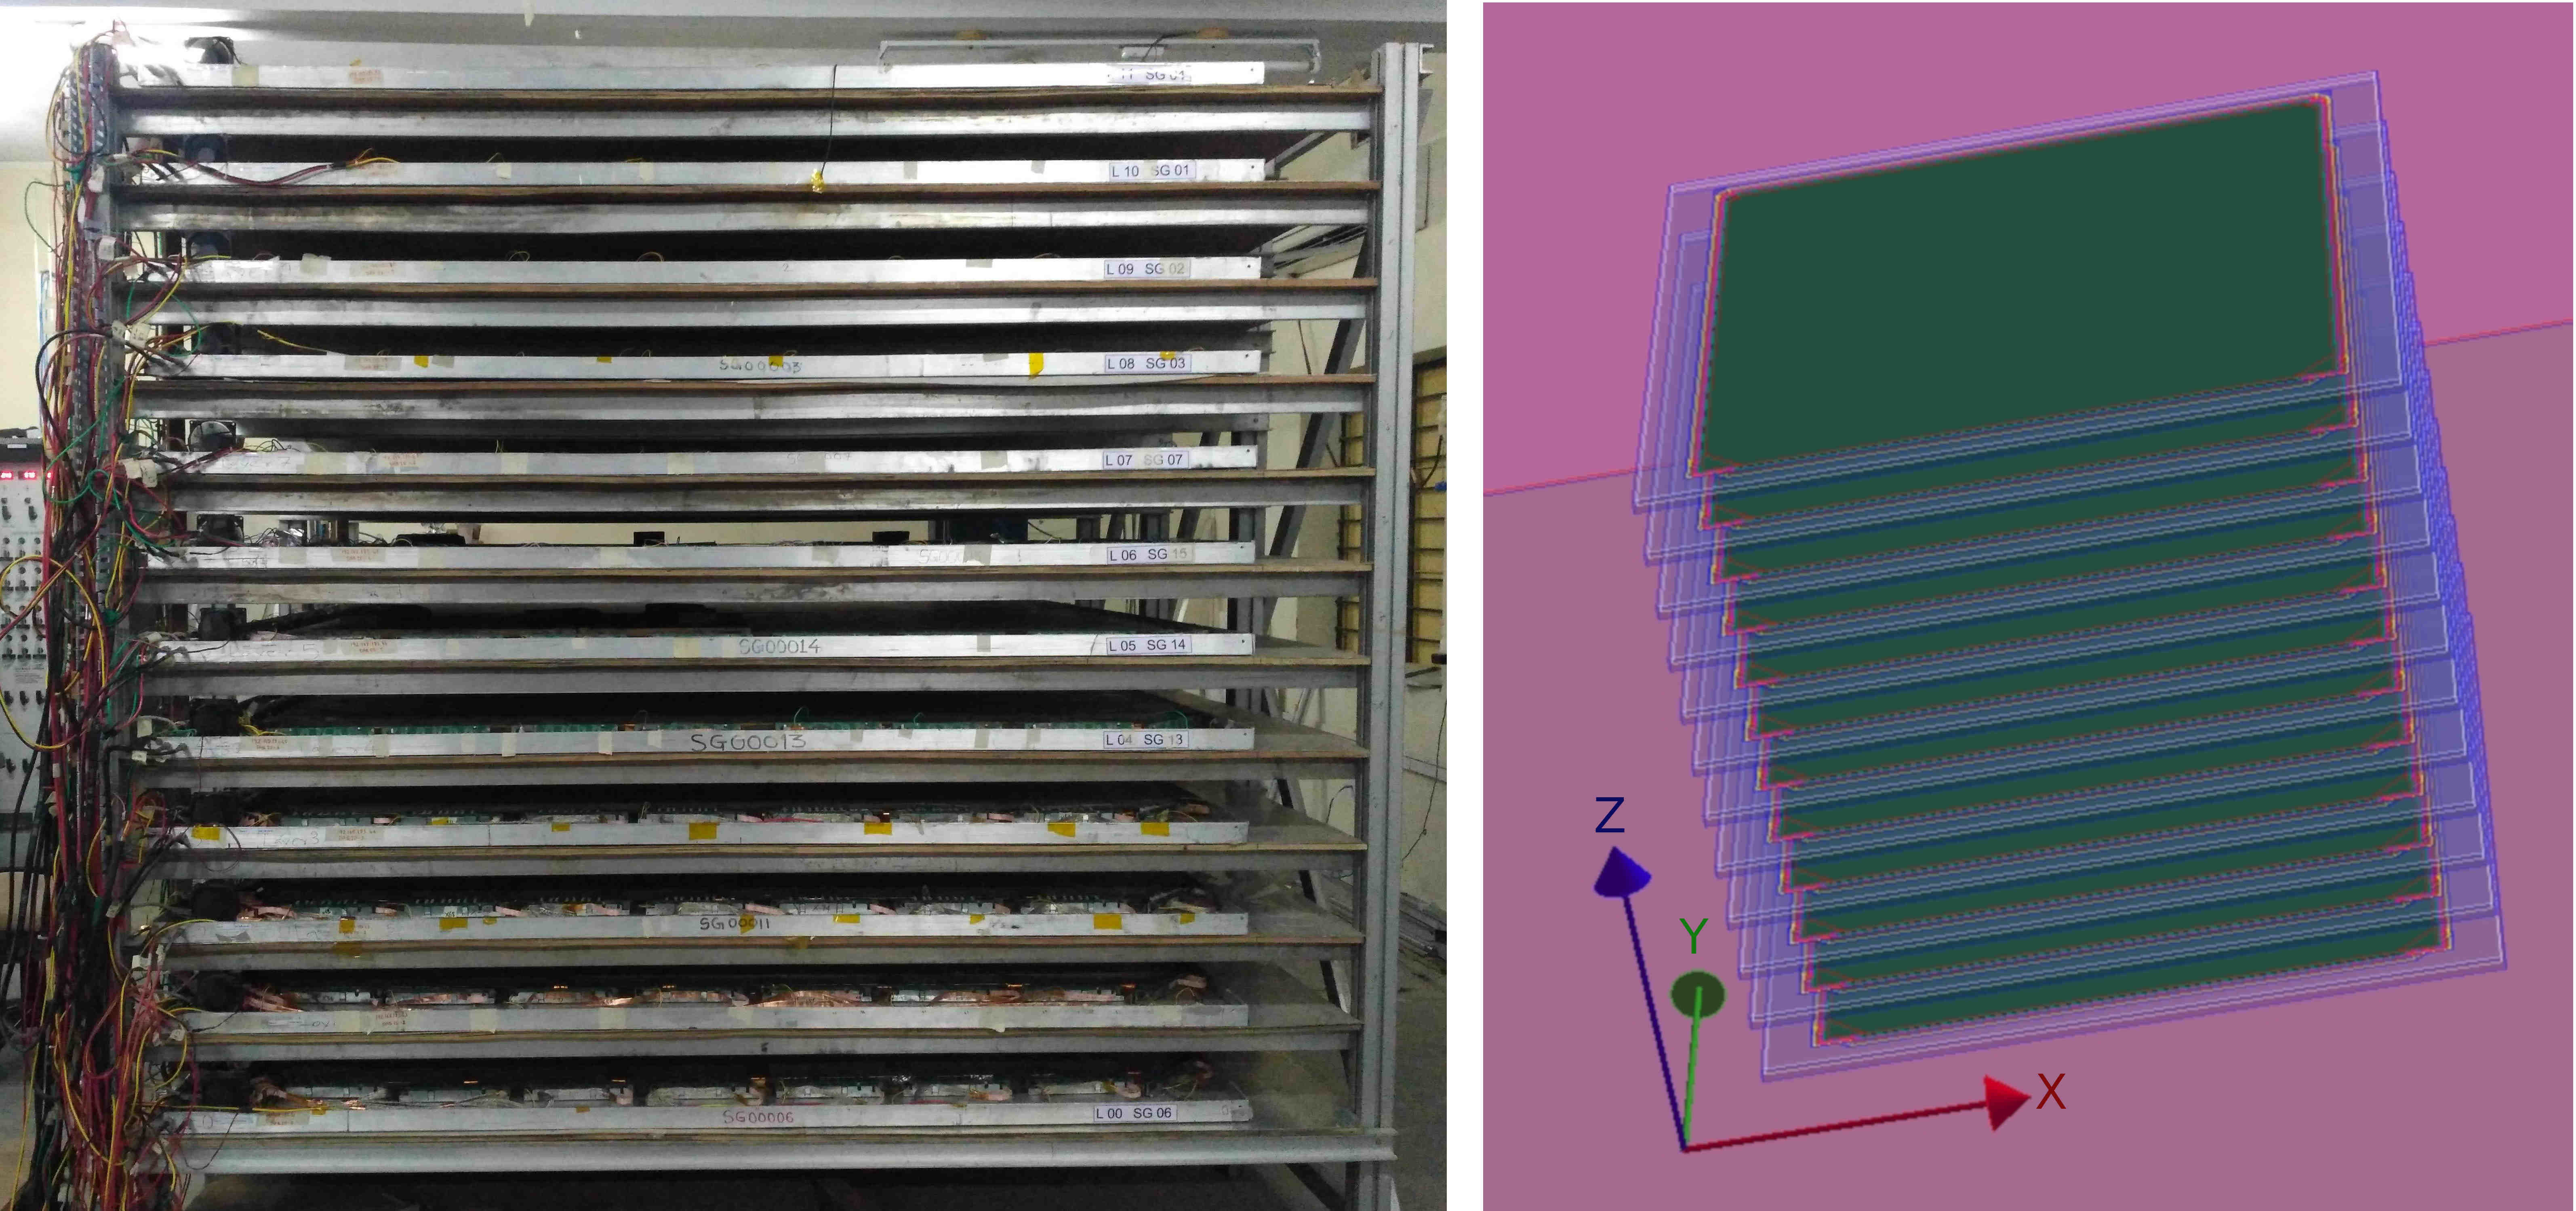
\includegraphics[width=0.99\linewidth]{ABlockStackiDAQ_new.jpg} 
  \caption{The detector stack with 12 layers of RPCs where the
    $X$-axis of the detector is making an angle of $-10^\circ$ with
    the geographic south, (left) experimental setup and (right) Geant4
    detector geometry of stack.}
  \label{fig:stack}
\end{figure}
An RPC gap is made of two glass electrodes of thickness 3\,mm with
a gap of 2\,mm between them. Uniform gap between these two electrodes
is maintained using a array of 2\,mm thick poly-carbonate buttons.
The glass gap is sealed on the outer edges to make it air-tight.
A non-flammable mixture of gas is continuously
flown inside the glass gaps through strategically placed nozzled.
This mixture of gasses serves as the active medium of the detector.
The RPCs are operated in avalanche mode. In this case, the mixture of
gases consists of R134a (95.2\%), iso-C$_4$H$_{10}$ (4.2\%) and
SF$_6$ (0.3\%). Both the outer surfaces of the glass gap are coated
with a thin layer of graphite. The RPCs are operated by applying
a differential supply of $\pm$\,5\,kV to the graphite layers to
achieve the desired electric field. The target gas inside the RPCs get
ionised by the transit of charged particles. This ionisation eventually
evloves into a avalanche in the presence of the high electric field
between the glass elctrodes. The avalanche in the RPCs induces
signals in the two orthogonal pickup panels placed on both sides of
the glass gaps labeled as X-side and Y-side. The pickup
panels are made of parallel copper strips of width 28\,mm with 2\,mm
gap between two consecutive strips. The RPCs used in this detector
stack are of the size of 1790\,mm\,$\times$\,1890\,mm. There are
60 strips on the X side and 63 strips on the Y side for each layer.

The induced signals from the pickup strips are amplified and
discriminated by a charge sensitive NINO\cite{nino} front-end
amplifier-discriminator board. Only in layer 11 (topmost layer),
ANUSPARSH front-end ASIC\cite{anusp} which is a CMOS, 8-channel,
high speed, low power amplifier-discriminator designed for
avalanche mode of operation for RPCs is used to study its performance.
The discriminated signals from these front-end boards are passed
to the FPGA-based RPCDAQ-board. The individual signals from every 
8$^{th}$ strips are \emph{OR}ed to get pre-trigger signals (S0 to S7).
The 1-fold (S0+S1+...S7), 2-fold (S0.S1+S1.S2+..S6.S7),
3-fold (S0.S1.S2+....S5.S6.S7) and 4-fold
(S0.S1.S2.S3+....S4.S5.S6.S7) signals created by RPCDAQ are passed
to the Trigger system module via Signal Router Board. The Global
Trigger is generated by Global Trigger Logic Board based (GTLB)
on X- or Y-plane with at least one strip hit within
100\,ns coincidence window. The coincidence is done for X and Y plane
independently and the final trigger can be generated by GTLB by OR
of Trigger in X- or Y-plane. The event signals in the RPCDAQ board
stretched to 1\,$\mu$s to overcome trigger latency from Trigger System
to RPCDAQ. Based on the arrival of trigger signals to RPCDAQ,
the event signals are latched and sent to the Data Concentrator
and Event Builder via Network Switch. The flow of signals from the
RPCs to the Back-End is shown in Figure~\ref{fig:sigflow}.
\begin{figure}[h]
  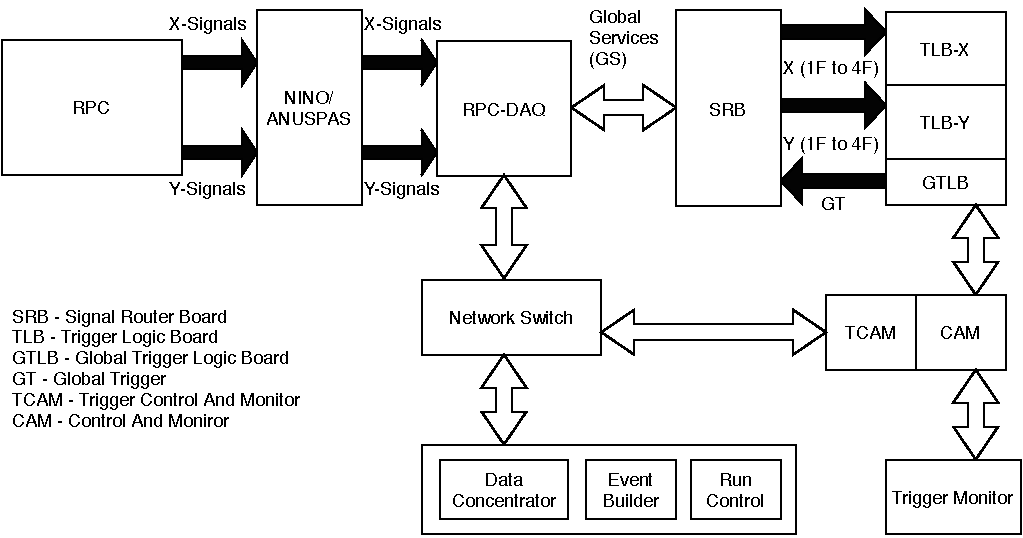
\includegraphics[width=1.0\linewidth]{DAQSchemeNewElectronics.pdf} 
  \caption{Signal flow from RPC to Back-End.}
  \label{fig:sigflow}
\end{figure}
The detailed description of signal processing and the Data Acquisition
system (DAQ) can be found in \cite{elec1}. The 1-Fold signals
from layers 4, 5, 6 and 7 are used as trigger to record the cosmic
events used in the present work.

Although the coincidence window is 100\,ns, event as well as noise
signals in a time window of 800\,ns after generation of the trigger
are also recorded due to stretching of the event latch. An event
typically contains strip hit and timing information of an event.
The strip hit is basically one logic bit per strip indicating
the signal in that strip is above the threshold value for each strip.
The timing data is consists of 16 time signal for each layer where
each TDC channel records time signals coming from every alternating
8$^{th}$ strips on one side of the layer.
The cosmic events recorded in the detector for the total observation
period of $\sim$\,17\,days between August 23, 2017, to September 8,
2017, with a trigger rate of $\sim$230\,Hz are used for the analysis.

\section{Monte-Carlo Simulation} \label{sec:montecarlo}
The Monte-Carlo Simulation for this study has been executed in
two stages. The Extensive Air Shower (EAS) has been simulated
by the CORSIKA simulation package. The information of daughter
particles generated by the EAS at the surface level has been
extracted and used as the input to the detector simulation.
The detector simulation has been performed using the GEANT4 toolkit. 
